% !TEX encoding = UTF-8 Unicode
%!TEX root = thesis.tex
% !TEX spellcheck = en-US
%%=========================================
\chapter{Security measures against manipulation by bots}
%title sucks, will change later.
\small{By Jan Samuelsen Lindemann}
\addcontentsline{toc}{section}{Management Summary}
\section*{Management Summary}
%mange forskjellige typer ting
%mange forskjellige løsninger
%en blanding av de forskjellige løsningene er nødvendig
%for å møte et sammensatt/komplekst trusselbilde
We are no longer living in a world where the internet is a somewhat obscure thing that only very few people use. Businesses are dependent on the communication opportunities that social networks on the internet provides, however with these opportunities comes many risks, such as automatic bots that will take action towards your social network or from your own devices toward another entity.
In the following chapter we have looked at many of the available security measures that can be used to reduce the risk you are exposed to from automatic bots, from many different points of view.
We explain some of the actions available for both a business or person being used as a unwitting agent in a botnet and for a entity being targeted by it.
The available options are presented with real world examples from companies and governmental institutions like Facebook, Europol, FBI and more.
Implementing the different measures will have an impact on how exposed the organization is to a potential botnet or infection, by reducing the potential benefits from running a botnet while increasing the cost of having the botnet active, your organization will become a less attractive target for many malicious entities.
The correct security measure for you and your organization is dependent on many factors, and there is not 1 cookie cutter solution that works for every scenario.
Size, technology and resources available will limit the measures that are available, while type of business, and what impact a botnet would have on your business will also be a deciding factor.
In the conclusion we recommend that cooperation between your organization and available governmental organizations such as national or sector CERTs, police organizations such as Europol or other national police as well as service providers such as ISPs can have great effect, especially in situations that cross borders or otherwise are out of your organizations control.
\newpage
\addcontentsline{toc}{section}{Abstract}
\section*{Abstract}
In this chapter we will go through some of the countermeasures available against botnets.
We will present approaches from different perspectives such as internet service providers, users, social network societies and others. We will where applicable include some examples of where these countermeasures have been used and to what effect.
In the end we will go over a conclusion on what can be learned from this and how it may apply to you.



%\section{Background}
%litt historie
%litt forskjellige typer? nevne torpig ettersom vi går inn på det i countermeasures?
%Litt forskjellige perspektiver?
%Mål disse forskjellige typene/perspektivene har?
%Metoder som benyttes
%%=========================================



\section{Countermeasures}
There are several different methods to counteract a botnet, depending on the perspective you take.
From the perspective of a user some countermeasures are viable, while there are different measures available as a ISP or a web host
In the following sections we will go through these different perspectives and describe the countermeasures available.
Many of these measures are gathered from real-world examples of dealing with botnets, from law enforcement like the FBI and Europol to social media network sites such as Facebook.
The different methods of acting against a botnet are often dependent on each other and will only have an effect if several measures from the different parts act together, from the user, via the internal departments responsible for implementing and handling security measures to third parties like law enforcement or other public institutions like CERTs.

\subsection{User}
As a user it is important to be aware of the risks inherent with the use of certain services and systems, nowadays malicious code can be delivered through a multitude of vectors, from exploit kits which require little to no interaction from the user to phishing emails that try to fool the user into accessing a malicious site or running a attachment that will infect the users system \cite{jan-brewer}. 
Paying attention to what the user is being asked to do and thinking twice if this actually makes sense can thwart many attempts at infecting the users system, many infection campaigns will pretend to be a legitimate request from a known company or service provider, as seen in a Torrentlocker campaign targeting norwegian users in 2015 \cite{jan-nsm-ransomware}, where the user would receive a email claiming to be from the norwegian post-office and asking the user to check a package delivery notice, the users system would then be infected with the Torrentlocker Ransomware that would encrypt files and ask for bitcoins as ransom for decrypting the files again. 
\\

Another infection vector is the exploitation of vulnerabilities in the software on the users system, either by attempting to get the user to manually execute a seemingly legitimate file that will exploit a vulnerability in the software used to open it or through exploit kits.
Exploit kits are tools used to serve as a platform for delivering malicious software for customers to their victims, they exploit vulnerabilities in software such as browsers or browser plug-ins like flash or java \cite{jan-kotov-ek}. Studies from 2013 show that around 70\% of the exploit kit traffic in Q4 2012 originated from Russia, China and Brazil\cite{jan-ek-source}, Russia and China being 2 countries that not necessarily are countries that will voluntarily cooperate with western countries when it comes to cybercrime investigation.  The victims are usually directed to a exploit kit from a legitimate website that has been modified by an attacker to silently redirect the victims browser to a malicious web-server, see figure~\ref{jan-ek-infection} for a common infection chain. By keeping software such as your browser and its plugins up to date or disabling them if not needed can mitigate or completely remove some of the risks associated with exploit kits and drive-by-downloads. Keeping software such as PDF-readers and other commonly used software updated will of course help.


\begin{figure}
	\centering
	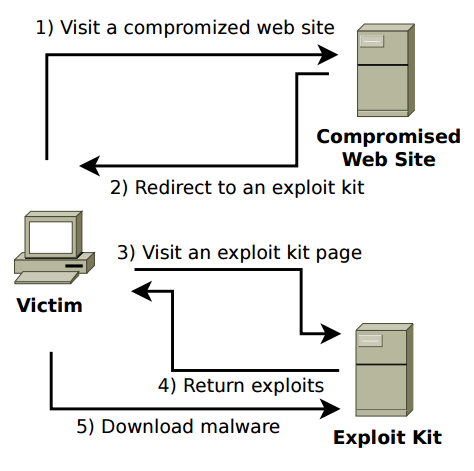
\includegraphics[scale=0.4]{fig/jan-ek-inf}
	\caption{Exploit kit infection scheme from \cite{jan-kotov-ek}.}
	\label{jan-ek-infection}
\end{figure}

\subsection{Institution}%evt. Business?
As a institution or business there are a few ways to reduce the risk associated with botnets or malware infection, depending on the policy regarding usage of computer resources and responsibility of these, measures may vary from business to business.
Keeping software updated is helpful as mentioned, but application whitelisting is not a new concept \cite{jan-mansfield-whitelist}. Instead of blacklisting known bad things the way a anti-virus solution would work we instead only allow known good applications to run, we see implementations of this in Apples iPhone where only applications approved by apple are allowed to run or in Windows AppLocker \cite{jan-windows-applocker} for windows 7 and newer. By limiting the approved applications for a user or a group of users one can limit the attack surface they expose.
Whitelisting network protocols is another way to limit the impact a botnet could have in network, by only allowing certain protocols to communicate a potentially infected computer may not be able to communicate with its command and control server. Similar to this is the act of network traffic inspection, rule based IDS or IPS solutions can look for known attributes in the network traffic and either block or alert when a match is found, in cases where the traffic pattern generated by the download of the malicious code of the bot is known, one can stop the infection before it happens. 




\subsection{Service provider}
Some botnets use a client-server architecture where several clients, or bots, are controlled by a centralized server. To communicate with these servers today where IP-addresses can change often the botnets will use DNS to figure out which IP-address to contact. Sinkholing is the act where you are deliberately sending the wrong IP-address in response to certain queries and end up directing the traffic from the original command and control infrastructure of the botnet to a server controlled by someone else.
This was used by Stone-Gross et al. \cite{jan_stone-gross} when they took over control of the Torpig botnet for several days in early 2009. Torpig was a botnet delivered through Mebroot, which replaced the master boot record of the infected system, a hard to detect rootkit. Mebroot in itself had no malicious function, but delivered other malware as a service. Torpigs victims where infected  through vulnerable web servers which had been exploited by the people behind mebroot. The victims browser would launch a malicious javascript that had been injected into the vulnerable web server which would perform a drive by download on to the victims system, which would infect the system with the mebroot rootkit and add it to the mebroot botnet, which could then download and install Torpig as a module and add the system to the Torpig botnet. \\


A somewhat controversial case of sinkholing domains associated with malware traffic is the case from 2014 where Microsoft got permission to sinkhole traffic towards several domains belonging to Vitalwerks Internet Solutions, the company behind no-ip, a dynamic dns provider. This was later overturned when the sinkholing proved to affect both legitimate and illegitimate use of the domains \cite{jan-microsoft-no-ip}. 
The use of sinkholing does however depend on the domain(s) being under the jurisdiction of a country that will cooperate with law enforcement in whichever country that is seeking action towards specific botnets and their associated domains. Since many of the command control servers utilize services known as bulletproof hosting this can prove difficult. As with exploit kits, many bulletproof hosters are in countries that are less inclined to act on cybercrime targeting foreign countries, however in july 2016 it was reported that several asian countries met to discuss the potential for forming a "Europol-style agency to fight cybercrime"\cite{jan-asia-europol}.

In Cooke et al.\cite{jan-usenix-botnet} they describe botnets using IRC-traffic, as a service provider this means that a botnet could be detected by inspecting the traffic from a network and look for known attributes belonging to a botnet, for instance IRC commands. By infiltrating the IRC channels used by the botnet one can learn of clients that are infected and by looking for DNS lookups of domains associated with the IRC networks one can find clients in ones network that is infected. IRC traffic is usually unencrypted, but can take advantage of for example ssl encryption to mask its own traffic and increase the technical challenge of detecting the traffic.

As technology evolves, so does the botnets with them,  Stone-Gross et al. \cite{jan_stone-gross} describe a botnet named Storm, that  utilized p2p to communicate. Detecting and stopping traffic from new botnets can be achieved by using honeypots and generating signatures based on observed traffic, this is the objective of Honeycomb project \cite{jan-Kreibich}. Honeypots are systems set up by a security researcher or organization to lure in malicious activity from hackers or automated bots, these often contain intentionally vulnerable systems that often appear to contain sensitive or otherwise interesting data or information, so they appear extra enticing for a hacker. By analyzing the commands and patterns of the traffic and actions perpetrated by the attacker one can learn of potentially new vulnerabilities the attacker attempts to leverage or other information such as command and control servers or just in general what the attacker will attempt to perform on a compromised system.


\subsection{Social network}

As described in \cite{jan-fis} the facebook immune system is a system that uses something they call the adversarial cycle(See figure~\ref{jan-adv-cycle-fis}), where the life cycle of the immune system is laid out.
Defending against a attack has a result that is detected by the attacker which then mutates his attack to counteract the defense mechanism. The goal of the defender is to lengthen the time it takes for the attacker to counter the defense mechanism, this increases the cost of the attacker and thus reduces how profitable attacking the social network is. In the facebook immune system they emphasize targeting features with high cost, due to them being hard to detect or change. This can mean targeting infrastructure such as the hosts IP address which can force them to relocate or use proxy services or it can for instance mean implementing tasks that cant be easily automated or not automated at all. Captcha \cite{jan-captcha} is one way to increase the costs of automation, while there exists services that solve captchas for money they cut into already not so great profits \cite{jan-boshmaf} and increasing complexity of captchas when detecting suspected malicious automated behavior could further increase cost for the attacker.


\begin{figure}
	\centering
	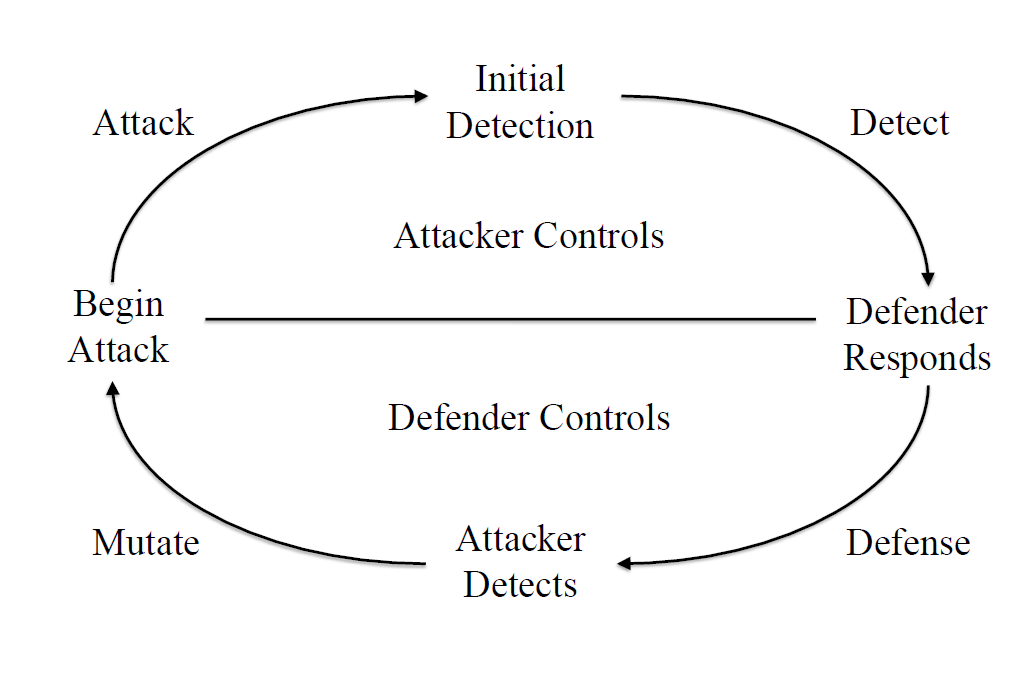
\includegraphics[scale=0.4]{fig/fis-adv-cycle}
	\caption{The adversarial cycle from \cite{jan-fis}.}
	\label{jan-adv-cycle-fis}
\end{figure}
\subsection{Law enforcement and government}
The facilitators of botnets and other malware are in most countries breaking the law with their operation since they are using computer resources without approval of the system owner, it follows that it should be in the interest of law enforcement to stop this activity. 
Due to the international and borderless nature of the internet, enforcing the law on a anonymous person behind a IP address is not a simple task. International co-operation is necessary to effectively take down the infrastructure of a botnet or prosecute the criminals behind it. Many botnets leverage the use of so called "bulletproof hosts" that reside in countries with a legal system that either has no laws at all regarding cybercrime or the laws are simply not enforced in cases where the victim is in another country. Many of these bulletproof hosts will often turn a blind eye towards the legality of the traffic their services are being used for.\\
The Convention on Cybercrime in 2001 attempted to target some of the issues with co-operation between countries and promoting a common criminal policy in relation to cybercrime (\cite{jan-coc}). The European Cybercrime Centre (\cite{jan-ec3}) is a part of Europol that focuses on cybercrime, by promoting cooperation between countries and between law enforcement agencies, private sector and academia.
An example of the results of cooperation between countries in taking down a botnet is seen when the FBI with the cooperation of law enforcement in other countries shut down and arrested the people and infrastructure behind the GameOver Zeus botnet in 2014 \cite{jan-fbi-GOZ, jan-fbi-GOZ2}. GameOver Zeus is p2p botnet targeting windows computers that is based on the code from the Zeus malware, it is thought to have infected up towards 1 million computers across the globe\cite{jan-krebs-goz}. The GameOver Zeus botnet is mostly spread through the Cutwail botnet. The takedown of the GameOver Zeus botnet was a cooperation between government agencies and private software security firms such as Dell, McAfee, Trend micro and many more.
%botnets all the way down.


\newpage
\section{Conclusion}
Depending on which perspective you look at problem from, your available options are different and by themselves they may not be available or be severely limited due to the specific circumstances surrounding your situation. Cooperation between the different groups may overcome this, it should be in the users interest that his place of work is not bothering or hindering his effectiveness in his daily tasks, just as it is in the internet service providers interest to limit the amount of illegitimate traffic going through its networks. Limiting the feasibility of running a botnet can not simply be done by one user, but is a team effort that requires every part of the chain, from the user on his computer to the business in charge of the network to the social network targeted by the botnet.
Increasing the cost while reducing the benefit of running a botnet will eventually make it economically unattractive to run a botnet for criminal organizations
\addcontentsline{toc}{section}{Self Evaluation}
\section*{Self Evaluation}
In the term paper i have tried to cover all the different security measures against a bot/botnet from various points of view. Most of the security measures are based on real-life cases or scholarly articles.
While there may not be a very high amount of articles about countermeasures towards social bots i believe that some of the countermeasures against common malware or other unauthorized software still applies.
I have tried to structure the paper into a logical order where the security measures from the various perspectives are presented, but some of the countermeasures overlap.
I've tried to keep the language to a non technical level that is easy to understand for the reader without a technical background. 
While i believe i covered the different countermeasures towards a social botnet well, in retrospect I believe i could have gone more into the costs associated with the different countermeasures, this would perhaps have given me more fleshed out paper.
However that is not something I initially planed to do and based on the initial feedback I believe I covered the topic without going into technical details, but in hindsight the cost of the countermeasures seems somewhat important.
Based on this I think that my work may warrant a "B" or "C".
